%!TEX root = ../main.tex
%%%%%%%%%%%%%%%%%%%%%%%%%%%%%%%%%%
% Links:
%
% Difficulty:
% Companies: 
%%%%%%%%%%%%%%%%%%%%%%%%%%%%%%%%%%

\chapter{TITLE OF THE CHAPTER}
\label{ch:mirror_binary_tree}
\section*{Introduction}

\section{Problem statement}
\begin{exercise}
	Write a function that given a binary tree, return mirror copy of it.

	\begin{example}
		\hfill \\
		Given the binary tree shown in Figure \ref{fig:mirro_binary_tree:example1} the function returns a tree like the one in Figure \ref{fig:mirro_binary_tree:example1_1}
		\label{ex:mirro_binary_tree:example1}.
	\end{example}

	\begin{example}
		\hfill \\
		Given the binary tree shown in Figure \ref{fig:mirro_binary_tree:example2} the function returns a tree like the one in Figure \ref{fig:mirro_binary_tree:example2_1}
		\label{ex:mirro_binary_tree:example2}
	\end{example}

	\begin{example}
		\hfill \\
		Given the binary tree shown in Figure \ref{fig:mirro_binary_tree:example3} the function returns a tree like the one in Figure \ref{fig:mirro_binary_tree:example3_1}
		\label{ex:mirro_binary_tree:example3}
	\end{example}
\end{exercise}


\begin{figure}
	\centering
	\begin{subfigure}[b]{0.25\textwidth}
	   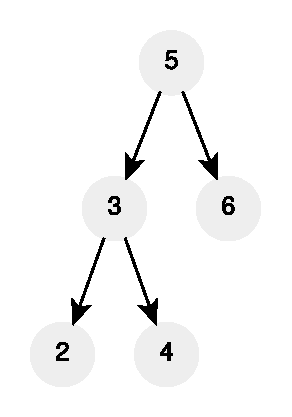
\includegraphics[]{sources/mirror_binary_tree/images/example1}
	   \caption{Input binary tree for the Example \ref{ex:mirro_binary_tree:example1}.}
	   \label{fig:mirro_binary_tree:example1}
	\end{subfigure}
	\hfill
	\begin{subfigure}[b]{0.4\textwidth}
	   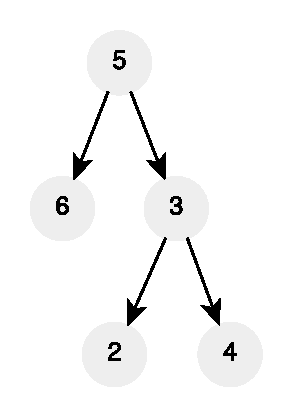
\includegraphics[]{sources/mirror_binary_tree/images/example1_1}
	   \caption{Output binary tree for the Example \ref{ex:mirro_binary_tree:example1}.}
	   \label{fig:mirro_binary_tree:example1_1}
	\end{subfigure}
	\centering
	\begin{subfigure}[b]{0.4\textwidth}
	   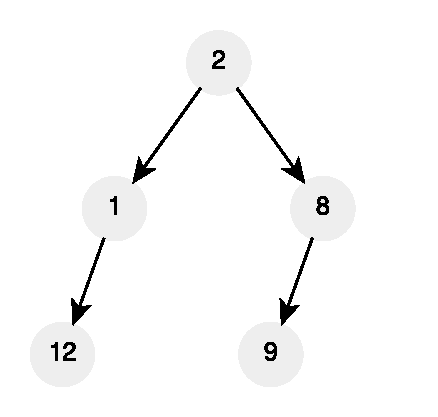
\includegraphics[]{sources/mirror_binary_tree/images/example2}
	   \caption{Input binary tree for the Example \ref{ex:mirro_binary_tree:example2}.}
	   \label{fig:mirro_binary_tree:example2}
	\end{subfigure}
	\hfill
	\begin{subfigure}[b]{0.4\textwidth}
	   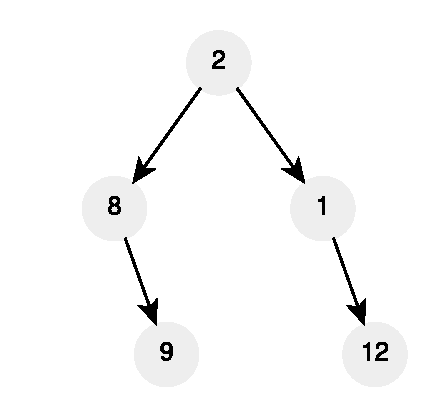
\includegraphics[]{sources/mirror_binary_tree/images/example2_1}
	   \caption{Output binary tree for the Example \ref{ex:mirro_binary_tree:example2}.}
	   \label{fig:mirro_binary_tree:example2_1}
	\end{subfigure}
	\centering

	 \caption[]{Input and output for Examples \ref{ex:mirro_binary_tree:example1} and \ref{ex:mirro_binary_tree:example2}}
\end{figure}


\begin{figure}
	\centering
	\begin{subfigure}[b]{0.4\textwidth}
		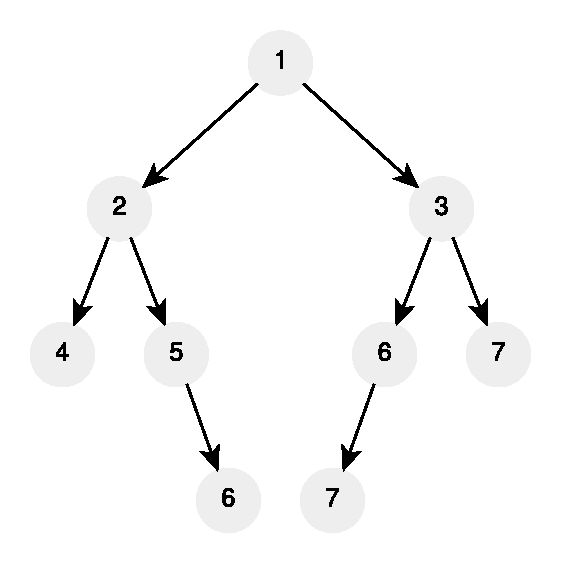
\includegraphics[]{sources/mirror_binary_tree/images/example3}
		\caption{Input binary tree for the Example \ref{ex:mirro_binary_tree:example3}.}
		\label{fig:mirro_binary_tree:example3}
	 \end{subfigure}
	 \hfill
	 \begin{subfigure}[b]{0.4\textwidth}
		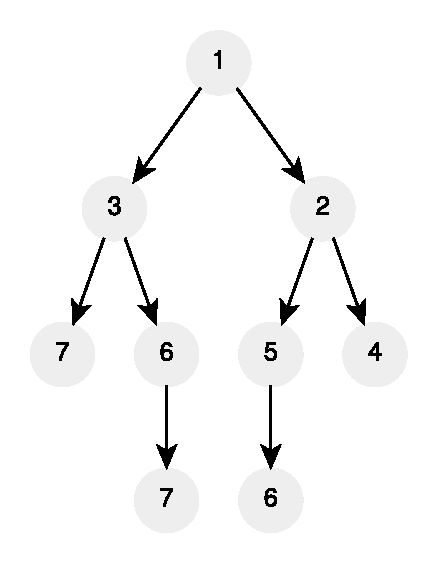
\includegraphics[]{sources/mirror_binary_tree/images/example3_1}
		\caption{Output binary tree for the Example \ref{ex:mirro_binary_tree:example3}.}
		\label{fig:mirro_binary_tree:example3_1}
	 \end{subfigure}
	 \caption[]{Input and output for Example \ref{ex:mirro_binary_tree:example3}}

\end{figure}




\section{Clarification Questions}


\begin{QandA}
	\item 
	\begin{answered}
		\textit{}
	\end{answered}
	
\end{QandA}

\section{Discussion}
\label{mirror_binary_tree:sec:discussion}
Let's start our discussion by trying to understand what it mirror copy really means. 
If we have a tree $T$ rooted at node $n$ then its mirror image \rotatecharone{$T$} is defined as follows:
\begin{itemize}
	\item \textbf{if $n$ has no children:} return  $T$. See node $9$ in the example \ref{ex:mirro_binary_tree:example2}.
	\item \textbf{if $n$ has one only the left child $n_l$:}  return $T$ having as left child the a mirrored copy of $n_l$.
	\item \textbf{if $n$ has one only the left child $n_r$:}  return $T$ having as right child the a mirrored copy of $n_r$]
	\item \textbf{if $n$ has both children:} return $T$ having as left child the mirrored copy of its right child $n_r$ and,
	 as right child the mirrored copy of its left child $n_l$.  An example of this case can be found
	  in the node $5$ in the Example \ref{ex:mirro_binary_tree:example1}
	 where its left and right children are first mirrored individually and then swapped. 
\end{itemize}
This recursive definition can be refined into the following idea. We can turn a tree $T$ rooted at $n$ into its mirror image
if we first mirror its children individually and only then we swap them.
Listing \ref{} shows an implementation of such idea.
\lstinputlisting[language=c++, caption={Sample Caption},label=list:mirror_binary_tree]{sources/mirror_binary_tree/mirror_binary_tree_solution1.cpp}

